\begin{flushright} {\tiny {\color{gray} basis\_p2p\_2D.tex}} \end{flushright}
%~~~~~~~~~~~~~~~~~~~~~~~~~~~~~~~~~~~~~~~~~~~~~~~~~~~~~~~~~~~~~~~~~~~~~~~~~~~~~~~~~~~~~~~~~~~~~~~~~~

This is used by the Crouzeix-Raviart element, see Section~\ref{sec:crouzeix-raviart}. 
\index{general}{Crouzeix-Raviart}


\begin{flushright} {\tiny {\color{gray} (tikz\_P2.tex)}} \end{flushright}
%~~~~~~~~~~~~~~~~~~~~~~~~~~~~~~~~~~~~~~~~~~~~~~~~~~~~~~~~~~~~~~~~~~~~~~~~~~~~~~~~~~~~~~~~~~~~~~~~~~

\begin{center}
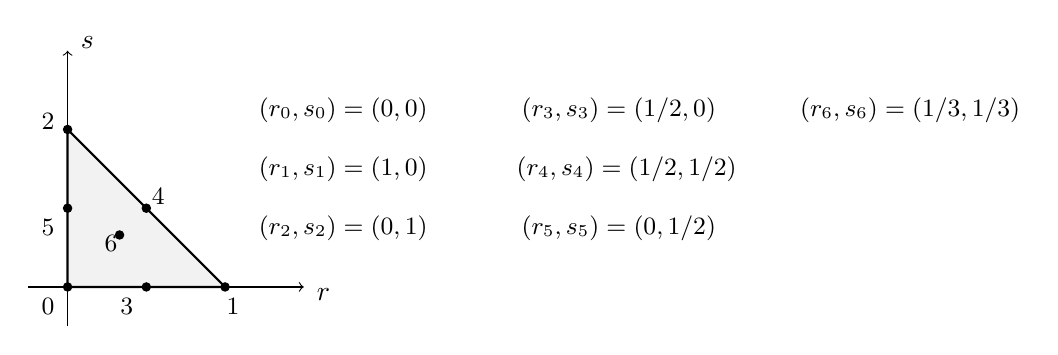
\begin{tikzpicture}
%\draw[step=0.5cm,gray,very thin] (0,0) grid (4,4); 
\draw[fill=gray!10,gray!10] (0.5,0.5)--(2.5,0.5)--(0.5,2.5)--cycle;
\draw[thick] (0.5,0.5)--(2.5,0.5)--(0.5,2.5)--cycle;
\draw [->] (0,0.5) -- (3.5,0.5);
\draw [->] (0.5,0) -- (0.5,3.5);
\node[] at (3.75,0.4) {$r$};
\node[] at (0.75,3.6) {$s$};
\draw[black,fill=black] (0.5,0.5)   circle (1.5pt);
\draw[black,fill=black] (2.5,0.5)   circle (1.5pt);
\draw[black,fill=black] (0.5,2.5)   circle (1.5pt);
\draw[black,fill=black] (1.5,0.5)   circle (1.5pt);
\draw[black,fill=black] (0.5,1.5)   circle (1.5pt);
\draw[black,fill=black] (1.5,1.5)   circle (1.5pt);
\draw[black,fill=black] (1.16,1.16) circle (1.5pt);

\node[] at (0.25,0.25) {\small $0$};
\node[] at (2.6,0.25)  {\small $1$};
\node[] at (0.25,2.6)  {\small $2$};
\node[] at (1.25,0.25) {\small $3$};
\node[] at (1.65,1.65) {\small $4$};
\node[] at (0.25,1.25) {\small $5$};
\node[] at (1.05,1.05)   {\small $6$};

\node[] at (4,2.75) {\small $(r_0,s_0)=(0,0)$};
\node[] at (4,2)    {\small $(r_1,s_1)=(1,0)$};
\node[] at (4,1.25) {\small $(r_2,s_2)=(0,1)$};
\node[] at (7.5,2.75) {\small $(r_3,s_3)=(1/2,0)$};
\node[] at (7.6,2)    {\small $(r_4,s_4)=(1/2,1/2)$};
\node[] at (7.5,1.25) {\small $(r_5,s_5)=(0,1/2)$};
\node[] at (11.2,2.75) {\small $(r_6,s_6)=(1/3,1/3)$};
\end{tikzpicture}
\end{center}



The basis functions are given by:
\todo[inline]{find reference}

\begin{mdframed}[backgroundcolor=blue!5]
\begin{eqnarray}
\bN_0(r,s) &=&  (1-r-s)(1-2r-2s+ 3rs) \\
\bN_1(r,s) &=& r (2 r -1 + 3s-3rs-3s^2 ) \\
\bN_2(r,s) &=& s (2s -1 + 3r-3r^2-3rs )\\
\bN_3(r,s) &=& 4(1-r-s)r(1 -3s ) \\
\bN_4(r,s) &=& 4rs [-2+3r+3s]\\
\bN_5(r,s) &=& 4(1-r-s)s(1-3r)\\
\bN_6(r,s) &=& 27 (1-r-s)rs 
\end{eqnarray}
\end{mdframed}
It is then easy to verify that for all basis functions we have 
$\bN_i(r_j,s_j)=\delta_{ij}$ where $j$ denotes one of the seven nodes. 
The derivatives are as follows:
\begin{eqnarray}
\frac{\partial \bN_0}{\partial r}(r,s) &=& r(4-6s)-3s^2+7s-3\\
\frac{\partial \bN_1}{\partial r}(r,s) &=& r(4-6s)-3s^2+3s-1\\
\frac{\partial \bN_2}{\partial r}(r,s) &=& -3s(2r+s-1)  \\
\frac{\partial \bN_3}{\partial r}(r,s) &=& 4(3s-1)(2r+s-1) \\
\frac{\partial \bN_4}{\partial r}(r,s) &=& 4s(6r+3s-2) \\
\frac{\partial \bN_5}{\partial r}(r,s) &=& 4s(6r+3s-4)\\
\frac{\partial \bN_6}{\partial r}(r,s) &=& -27s(2r+s-1)
\end{eqnarray}

\begin{eqnarray}
\frac{\partial \bN_0}{\partial s}(r,s) &=& -3r^2+r(7-6s)+4s-3\\
\frac{\partial \bN_1}{\partial s}(r,s) &=& -3r(r+2s-1)\\
\frac{\partial \bN_2}{\partial s}(r,s) &=& -3r^2+r(3-6s)+4s-1 \\
\frac{\partial \bN_3}{\partial s}(r,s) &=& 4r(3r+6s-4)  \\
\frac{\partial \bN_4}{\partial s}(r,s) &=& 4r(3r+6s-2) \\
\frac{\partial \bN_5}{\partial s}(r,s) &=& 4(3r-1)(r+2s-1)\\
\frac{\partial \bN_6}{\partial s}(r,s) &=& -27r(r+2s-1)
\end{eqnarray}

Note that the basis functions can also be expressed as a function of the barycentric coordinates, 
as in the MILAMIN code \cite{daks08} or in Cuvelier \etal (1986) \cite{cuss86}\footnote{Note
that the numbering of the nodes in the book is different with respect to the one above. }

\begin{eqnarray}
N_0(\lambda_1,\lambda_2,\lambda_3) &=& \eta_1(2\eta_1-1)+ 3\eta_1\eta_2\eta_3\\
N_1(\lambda_1,\lambda_2,\lambda_3) &=& \eta_2(2\eta_2-1)+ 3\eta_1\eta_2\eta_3\\
N_2(\lambda_1,\lambda_2,\lambda_3) &=& \eta_3(2\eta_3-1)+ 3\eta_1\eta_2\eta_3\\
N_3(\lambda_1,\lambda_2,\lambda_3) &=& 4\eta_2\eta_3 - 12\eta_1\eta_2\eta_3\\
N_4(\lambda_1,\lambda_2,\lambda_3) &=& 4\eta_1\eta_3 - 12\eta_1\eta_2\eta_3\\
N_5(\lambda_1,\lambda_2,\lambda_3) &=& 4\eta_1\eta_2 - 12\eta_1\eta_2\eta_3\\
N_6(\lambda_1,\lambda_2,\lambda_3) &=& 27\eta_1\eta_2\eta_3 
\end{eqnarray}

\todo[inline]{
VERIFY that when $\eta_1=1-r-s$, $\eta_2=r$ and $\eta_3=s$ we find the above $r,s$ basis functions
}


%1-4*eta1+3*eta1*eta3-3*eta2*eta3 ...
%-1+4*eta2+3*eta1*eta3-3*eta2*eta3 ...
%3*eta1*eta3-3*eta2*eta3 ...
%4*eta3+12*eta2*eta3-12*eta1*eta3 ...
%-4*eta3+12*eta2*eta3-12*eta1*eta3 ...
%4*eta1-4*eta2+12*eta2*eta3-12*eta1*eta3 ...
%-27*eta2*eta3+27*eta1*eta3

%1-4*eta1+3*eta1*eta2-3*eta2*eta3 ...
%+3*eta1*eta2-3*eta2*eta3 ...
%-1+4*eta3+3*eta1*eta2-3*eta2*eta3 ...
%4*eta2-12*eta1*eta2+12*eta2*eta3 ...
%4*eta1-4*eta3-12*eta1*eta2+12*eta2*eta3 ...
%-4*eta2-12*eta1*eta2+12*eta2*eta3 ...
%27*eta1*eta2-27*eta2*eta3];  


